%\begin{savequote}[8cm]
%Alles Gescheite ist schon gedacht worden.\\
%Man muss nur versuchen, es noch einmal zu denken.

%All intelligent thoughts have already been thought;\\
%what is necessary is only to try to think them again.
 % \qauthor{--- Johann Wolfgang von Goethe \cite{von_goethe_wilhelm_1829}}
%\end{savequote}

\chapter{Low convergence ratio implosions} \label{ch-lowCR}

\minitoc

\section{Introduction}

%Increasing the convergence ratio of an ideal (or one-dimensional) ICF implosion results in higher areal densities, and as such higher yields and gains. However, increased capsule convergence also leads to increased hydrodynamic instabilities, which results in experimental performance far below this predicted performance.

Implosions using wetted-foam capsules provide an opportunity to explore how fusion performance varies with convergence. The use of liquid DT rather than DT-ice means that capsules are fielded at higher temperatures (between 20 and 26 K), resulting in higher densities in the central vapour  region (between 0.6 and 4.0 \unit{\milli\gram\per\centi\meter\cubed}) \cite{Olson2016}), which in turn results in reduced capsule convergence. The convergence ratio of wetted-foam implosions can thus be controlled through the initial temperature of the capsule.

In an ideal ICF implosion, increasing the convergence ratio results in higher areal densities and increased gain. However, it is well-established that increasing the convergence ratio also leads to increased hydrodynamic instabilities, which prevents these high gains from being achieved experimentally. At low-convergence ratio the ideal performance is lower, but such instabilities are reduced: recent low-convergence ratio wetted-foam shots on the NIF demonstrated low amounts of instability, resulting in good agreement between experiment and simulation \cite{Olson2016, Zylstra2018}. 

In this chapter, one-dimensional (1D) simulations are performed to explore the possible fusion performance that could be obtained using low-convergence ratio implosions of wetted-foam capsules. First, a range of relevant previous results are discussed in Section \ref{sec: PreviousLowCRResults}. An expected low-instability regime is then identified (based on limits to convergence ratio and other key implosion parameters) so that 1D simulations are expected to be a reasonable estimate of experimental performance. A standard laser pulse sequence and capsule design are chosen and outlined in Section \ref{sec: CapsuleAndPulse}. These contain a number of `free' parameters, which are optimised for a number of different capsule sizes during a large-scale simulation campaign. Section \ref{sec: OptimisationCampaign} outlines how this simulation/optimisation campaign was performed, and the resulting `optimal' implosions over a range of different energies are presented and discussed in Section \ref{sec: LowCRResults}. Finally, the limitations of this approach are considered in Section \ref{sec: LowCRLimitations}, along with ways that it could be further developed in the future.

The purpose of this approach was to provide a first exploration of this parameter space, to determine whether IFE-relevant gains could be obtained with such implosions and what energies key milestones such as break-even or reactor level gains may require. The use of 1D simulations means that the predictions made are not likely to be exact. The performance achieved in such a regime will not match the high gains that are routinely simulated for higher-convergence ratio implosions; however, if significant performance can be obtained in these simulations, the low-instability nature of the regime and the greater-than-typical expected agreement between simulation and experiment may suggest an interesting possible direction for IFE research.

%In this chapter, the possible fusion yield of low-convergence ratio implosions of wetted-foam capsules is explored through a large-scale simulation campaign. A regime was identified (based on low-convergence ratio, alongside other implosion criteria) where instability growth is expected to be low, and one-dimensional simulations would provide a reasonable estimate of expected performance. This campaign was intended as a first exploration of what performance may be possible using such capsules at low-convergence ratio. While the gains of such capsules are expected to be lower than those simulated for high-convergence implosions, when the higher-than-typical expected agreement between simulation and experiment is considered it may be that the low-convergence ratio implosions could actually offer improved experimental performance. The simulation campaign presented consists of choosing a capsule design and laser pulse profile, and optimising a number of free parameters within this design to optimise the gain achieved for capsules at a range of different radii/energy-scales.

%Wetted-foam ICF capsules, consisting of a low-density foam saturated with liquid DT, can be used in place of conventional DT ice capsules. The use of liquid (rather than frozen) DT means that such capsules are fielded at a higher initial temperature, between 20 and 26K. This higher temperature leads to a higher density of DT vapour within the central void of the capsule, ranging between 0.6 and 4.0 \unit{\milli\gram\per\centi\meter\cubed} \cite{Olson2016}. Higher vapour densities lead to less capsule convergence, and thus varying the temperature of wetted-foam capsules provides an opportunity to explore how implosion physics varies with convergence.

%In ideal (1D) implosions, increasing the convergence ratio of the capsule leads to higher areal densities, and higher fusion yields. However, high convergence implosions are particularly susceptible to hydrodynamic instability growth, which results in significantly reduced experimental performance. Recent implosions of wetted-foam capsules at the NIF have demonstrated how using a lower convergence ratio can result in low instability growth, and therefore result in good agreement between experimental and simulated results \cite{Olson2016, Zylstra2018}.

%However, it is well established that low convergence implosions are less susceptible to hydrodynamic instability growth, and implosions of wetted foam capsules at the NIF demonstrated that this can result in good agreement between simulation and experiment  \cite{Olson2016, Zylstra2018}. Achieving high experimental yields thus is a balance of these two competing trends: as convergence ratio increases so do the ideal fusion yield, but the increase in instability growth leads to larger discrepancies between this predicted performance and experiment.

%In this chapter, the possible fusion yield of low-convergence ratio implosions of wetted-foam capsules is explored in a large-scale simulation campaign. A regime was identified (based on low-convergence ratio, and other implosion criteria) where instability growth is expected to be low, and one-dimensional simulations would provide a reasonable estimate of expected performance. This was intended as a first exploration of what may be possible in such a regime; if sufficiently high fusion performance could be obtained, it may be the case that this coupled with the higher-than-typical agreement between simulation and experiment in this regime may in fact outperform higher convergence implosions in experiments.

%In Section \ref{sec: PreviousLowCRResults}, the results of previous experiments and simulation efforts relevant to low-convergence implosions are discussed. In Section \ref{sec: Low-Instability} a range of different parameters influencing instability growth is considered - culminating in four criteria to minimise instability growth used to define this new regime, and thus (hopefully) ensuring that 1D simulations are reasonably accurate. The capsule design and laser pulse sequence that will be optimised in the simulation campaign is then considered in Section \ref{sec: CapsuleAndPulse}. The procedure followed in the simulation campaign is then discussed in Section \ref{sec: OptimisationCampaign}, before the results are presented in Section \ref{sec: LowCRResults}. Finally, the limitations of this approach are considered in Section \ref{sec: LowCRLimitations}, and ways that the work could be developed further are discussed.

%One of the promising possibilities that wetted foam capsules enable is a degree of control over the convergence ratio that is not possible with conventional capsules. Wetted-foam targets contain liquid DT wicked in a carbon foam. They are thus fielded at higher temperatures between 20 and 26 K (where DT is in liquid form), which in turn leads to higher vapour pressures ranging from 0.6 \unit{\milli\gram\per\centi\meter\cubed} to 4.0 \unit{\milli\gram\per\centi\meter\cubed}. These higher vapour pressures enable lower convergence ratios to be achieved. Not only this, but it also provides a way to control the convergence ratio largely independently from other implosion properties, by varying the temperature at which the capsule is fielded \footnote{Doing this has a small impact on some of the other properties, but this is essentially negligible.}. This enables the impact of convergence ratio on an ICF implosion to be explored.

%The first wetted foam target was shot on the NIF in 2016, in shot N160421. The results were interesting; neutron yield of \hl{VALUES} were achieved, which were promising and suggested a good level of performance could be achieved with these capsules. More promising however was the fact that agreement between the experimental and simulated results were high, suggesting a capsule that was performing roughly as expected, and without significant instability growth. Further shots presented by Zylstra \textit{et al.} confirmed this, and showed explicitly the link with convergence ratio. At low convergence ratio, the agreement with 2D simulations were very high, and as this increased the agreement rapidly began to get worse. 

%This raised the prospect of a new, alternative approach to ICF experiments. Previous approaches had targeted high convergence ratio implosions with very large gains, but failed to achieve them due to poor agreement with simulations - efforts were then ongoing to improve this agreement by reducing the instability growth. The alternative to this would be to operate at low-convergence ratio, in a regime where the agreement between simulation and experiment inherently appeared to be high. If performance could be explored in this regime in simulations and a high-performing design could be identified, then it could be reasonably expected that the experimental performance would also be high. The question was whether it would be possible to achieve sufficiently high performance at low convergence ratio to make such an approach worthwhile.

%The other benefit of this approach was that these low convergence ratio implosions were exhibiting low instability growth. This meant that the performance of such implosions could be reasonably well approximated as one-dimensional, allowing 1D simulations to be used to explore the performance. As 1D codes are relatively simple and quick to run (particularly compared to their 2D or 3D equivalents), this meant that a large-scale simulation campaign would be feasible.

%Such a campaign was therefore performed to explore the possible performance of wetted-foam capsules at low convergence ratio at a range of laser energies, and is described in this chapter. First, some of the previous results of low-convergence work is discussed, and the NIF shots are considered in further detail. Secondly, in an attempt to ensure instability growth is minimal and thus 1D simulations are accurate, other 1D implosion properties that correlate with instability growth are considered; a low-instability regime is thus identified which will set the boundaries for this campaign. Definitions of key parameters are then defined, describing the key metrics through which the simulated implosions will be judged.

%Section then discussed the form of the implosions considered, in terms of the laser profile and the capsule design. The simulation code and paramters used to simulate these implosions are then discussed in SECTION, before SECTION discusses how the simulation campaign was actually performed and conducted. The results achieved in this campaign are then presented and discussed in SECTION, before a discussion of the limitations of this campaign and the efforts taken to model the impact of these. Finally, a discussion on benchmarking of the code is included.

\section{Previous research into wetted-foam capsules and low-convergence ratio implosions} \label{sec: PreviousLowCRResults}

\subsection{Experimental results}

The first DT-wetted foam shot on the NIF (designated N160421) was performed in 2016, and was reported on by Olson \textit{et al.} \cite{Olson2016}. $(4.5 \pm 0.1) \times 10^{14}$ neutrons were generated, which suggested that a good level of performance could be achieved with such implosions. More impressive however was the close agreement between the simulation and experiment. 2D simulations were able to match a wide range of implosion metrics (including temperatures, bang time, hotspot radius and inferred pressures) to within the experimental error. These metrics were also very well described even by a 1D RAGE simulation (with a mix model included), which gave a ratio between experimental and simulated yield of nearly 80 \%. 

N160421, and subsequent wetted-foam shots N160626 and N161204, were then discussed by Zylstra \textit{et al.} \cite{Zylstra2018} in 2018. These three shots spanned a convergence ratio range of 12-20, and confirmed that convergence ratio could indeed be controlled through initial capsule temperature. These shots were again simulated using the HYDRA and xRAGE codes. The agreement was very good at low convergence ratio (with yield and ion temperature agreeing to within 5 \% for N160421 with a convergence ratio of 12), but as convergence increased the level of agreement was reduced, resulting in an experimental yield for the CR=20 shot that was only 30 \% of that predicted by the simulation. The intermediate shot, with a convergence ratio between 16 and 17, showed a good agreement of above 70 \%\footnote{It should be noted that the exact reason for these discrepancies could not be identified in \cite{Zylstra2018}.}. These NIF shots therefore showed that wetted-foam capsules could be used to generate low-convergence ratio shots on the NIF, and that the agreement with simulations at low-convergence ratio was relatively high.

This was not the first time a link between low convergence ratio and agreement with simulation was observed; the same result is highlighted in the following (non-exhaustive) collection of references \cite{Kato1996, Nishimura2000, Meyerhofer2001, Li2002, Lindl2004, LePape2014, Khan2016, Haines2017a}. This agreement was identified as far back as 1980 \cite{Key1980}, where it was observed that lower initial aspect ratios (thicker shells as a function of radius, resulting in lower implosion velocities and less convergence) resulted in performance that was more 1D-like. Two developments have led to increased recent interest in low convergence ratio implosions. Firstly, higher laser energies make it more feasible to achieve high gain in such a regime. Secondly, wetted-foam capsules (where the convergence ratio can be controlled through capsule temperature) mean that the convergence ratio of a capsule can be changed without substantial changes to the capsule, allowing it to be varied almost independently of other parameters.

While the NIF shots discussed so far were indirect-drive, similar links between convergence ratio and 1D-like performance have also been observed in direct-drive shots on Omega. Regan \textit{et al.} observed that the hotspot pressure and compressed areal density of capsules using DT ice layers (rather than wetted-foams) reached 90\% of the 1D simulated values for convergence ratios below 17 and adiabats greater than 3.5 \cite{Regan2016}. When the convergence ratio was increased past 17 a rapid drop-off occurred, which shows good qualitative agreement with the trend in yield observed on the NIF shots. This shows that this relationship applies for both indirect and direct-drive implosions, using both DT-ice or DT-wetted foam layers\footnote{It is also worth noting that that a low convergence ratio, high adiabat design using thin shells at high implosion velocities \cite{Williams2021} recently achieved the facility record neutron yield at Omega. These results were achieved after the work discussed in this chapter was performed.}.


\subsection{Simulation work} 

This topic has also been explored through simulation work. 2D simulations were previously used to investigate how the yield of wetted foam capsules changed with varying vapour density (and thus convergence ratio), for different amplitudes of a Legendre $P_4$ flux asymmetry. As expected, they found that the higher vapour density / lower convergence ratio implosions were significantly more robust to this asymmetry, with a higher ratio of 2D to 1D yield \cite{Olson2013}. Simulations performed in preparation for the NIF shots suggested that sensitivity to capsule instability growth and x-ray flux assymmetries increased with convergence ratio, leading to strong agreement between 2D and 1D simulations for CR=15 shots when surface roughness was applied, compared to much worse agreement for high convergence ratio shots - leading to a hypothesis that using low convergence ratios would lead to reduced instability growth and a robust predictive capability \cite{Olson2016a}. 

High resolution 2D xRAGE simulations performed in 2017 investigated full-scale wetted foam capsules with a variety of `asymmetry seeds'. These simulations showed that when surface roughness and drive asymmetries were included, yield increased with convergence ratio through the range of 12<CR<20. However, when the capsule support tent and fill tube were also included the yield was roughly constant as a function of convergence ratio up to CR=20, at which point it began to decrease \cite{Haines2017a}. The capsule support tent was found to be the main seed for this instability growth. Despite this, the paper concluded "as the level of these asymmetries is reduced, the wetted foam platform will enable layered implosions to be fielded at convergence ratios that optimize the trade-off between enhanced 1D performance and increased implosion instability as the convergence ratio is increased".

There are some differences between the simulations presented in \cite{Haines2017a} and the designs considered in this chapter, but these are unlikely to lead to significant changes in behaviour. For instance, while the use of a capsule support tent is specific to indirect-drive, direct-drive implosions require stalks to hold the capsule in place which will likely also have a significant effect. The effect of the stalk on direct-drive implosions is still being investigated; simulation work on this topic has suggested stalks are responsible for a yield degradation of 10-20\% \cite{Shah2017}, while more recent simulations indicated the impact of the stalk was significant but were unable to quantify it exactly \cite{GatuJohnson2020}. The other key difference between the low-convergence xRAGE simulations in \cite{Haines2017a} and the designs considered in this chapter is their use of a high-density carbon (HDC) ablator. Such ablators are typically more susceptible to the effects of the fill tube, but may be more robust to the capsule support tent compared to CH \cite{Zylstra2022, Abu-Shawareb2022, Haines2019a, Clark2018}.

A key observation from the xRAGE simulations in \cite{Haines2017a} was the impact of the first shock driven through the caspule. If the first shock is not strong enough to melt the HDC ablator, then then the  imprint from the support tent (and the HDC microstructure, which was not considered in \cite{Haines2017a}) may seed significant instability growth \cite{Mackinnon2014, Haines2019a}. The xRAGE simulations had a weak first shock, which was likely why the support tent led to such significant yield degradation \cite{Haines2017a}. Other xRAGE simulations using stronger initial shocks led to the support tent contributing to only a 1 \% reduction of the 2D yield \cite{Haines2019a}, highlighting that this can indeed be well mitigated using a strong first shock (this was also seen in the xRAGE simulations of N160421, the first liquid layer DT shot, with a higher adiabat). A number of developments since the 2017 xRAGE simulations were performed have also been implemented to reduce the amplitude of these asymmetry seeds. Alternative designs for supporting the capsule have been proposed \cite{Weber2017, Hammel2018a} and have led to improved capsule performance \cite{Hammel2018a}. In addition, the fill tube diameter has been significantly reduced since the 2017 simulations, leading again to less yield degradation \cite{Weber2020, Pak2020}. 2019 xRage simulations of a wetted-foam capsule with a plastic shell at CR = 19 showed good agreement with experiment \cite{Haines2019a}, suggesting that these instabilities can indeed be controlled (even at higher convergence ratios) if asymmetry seeds are well mitigated. 

 %Stalks have been shown to outperform silk-strings (the alternative capsule support for direct-drive), but still lead to significant yield degradation compared to experiment \cite{Igumenshchev2009}. The exact impact of capsule stalks has not been quantified to the same degree as support tents, and research into this is still ongoing. Simulation work has suggested that 10-20 \% yield degradation due to stalk, but did not observe differences in experiments between shots (but yield was much lower in all shots) \cite{Shah2017}, while more recent work suggested that the stalk is indeed important but could not quantify the effect on yield \cite{GatuJohnson2020}.
\subsection{Implications of these previous findings} 
The significance of these previous results are clear. The use of low-convergence ratio has been demonstrated in both simulations and in experiments to reduce instability growth, and as convergence ratio is increased yield degradation due to instabilities is also observed to increase. Detailed xRAGE simulations investigating the impact of convergence ratio \cite{Haines2017a} have demonstrated that low-convergence alone isn't sufficient to mitigate instability growth, but more recent simulations (and significant research effort to reduce the seeds of these instabilities) indicate that it is possible to control asymmetry seeds and thus the resulting instabilities can be minimised. The 1D simulations in this chapter do not include the effects of these asymmetry seeds, and thus it is important to note that these are also key to minimising instability growth.

%High resolution 2D xRAGE simulations performed in 2017 of full-scale wetted foam capsules including surface roughness and drive asymmetries found that yield increased with convergence ratio through the range of 12<CR<20, but found that when the capsule support tent and fill tube were included, the yield was roughly constant as a function of convergence up to CR=20, at which point it began to decrease \cite{Haines2017a}. This discrepancy was largely caused by the capsule support tent.

%However, a range of factors should be considered in interpreting this result. Recent NIF shots (including the DT wetted-foam shots) have used high-density carbon (HDC) shells; these have a higher density and thus higher ablative pressure than the previous plastic (CH) shells. HDC ablators are more susceptible to the effects of the fill tube, but are typically more robust to the capsule support tent compared to CH \cite{Zylstra2022, Abu-Shawareb2022, Haines2019a, Clark2018}. The caveat here is that the first shock should be strong enough to melt the HDC shell; otherwise, microstructures in the HDC may seed instability growth \cite{Mackinnon2014, Haines2019a}. The simulated design in the 2017 xRAGE simulations had a weak first shock, and the authors noted that this made these implosions particularly susceptible to instabilities seeded by the tent \cite{Haines2017a}; as demonstrated by the fact that xRAGE simulations of HDC ablator targets with stronger initial shocks demonstrate that the tent caused only a 1 \% reduction of the 2D yield \cite{Haines2019a}. The xRAGE simulations of N160421 (the first liquid layer DT shot, with a higher adiabat) also demonstrated a much smaller amount of yield degradation from this effect. 

%It's also worth noting the significant improvements that have been made since these 2017 simulations. Alternative designs for supporting the capsule have been proposed have been proposed \cite{Weber2017, Hammel2018a} and have led to improved capsule performance \cite{Hammel2018a}. In addition to this, the fill tube diameter has been significantly reduced since the 2017 simulations (the N210808 shot had a 2 \unit{\micro\meter} fill tube \cite{Abu-Shawareb2022}), leading again to less yield degradation and improved performance \cite{Weber2020, Pak2020}. These improvements may mean that some of the yield degradation observed in the 2017 simulations could be reduced, meaning that some increase in performance with convergence ratio (while staying in the CR<20 convergence ratio range discussed) may indeed lead to increased performance. This matches the conclusion made in that paper, which stated "as the level of these asymmetries is reduced, the wetted foam platform will enable layered implosions to be fielded at convergence ratios that optimize the trade-off between enhanced 1D performance and increased implosion instability as the convergence ratio is increased" - which is the intention of this chapter.

%Simulations of wetted foam with plastic shell at CR = 19 showed good agreement \cite{Haines2019a}, suggesting instabilities can be controlled. However, very conservative. Similar experiment with high asymmetry seeds showed significant yield degradation. When asymmetry seeds are suppressed (i.e. strong shock), then instability growth can be suppressed too.

%Stalks used for direct drive rather than tents. Initial simulation work suggested that stalks outperformed silk string, but still caused significant degradation \cite{Igumenshchev2009}. Simulation work suggested 10-20 \% yield degradation due to stalk, but did not observe differences in experiments between shots (but yield was much lower in all shots) \cite{Shah2017}. Recent work suggested that the stalk was indeed important, but could not quantify the effect on yield \cite{GatuJohnson2020}. Other simulations showed that lonw-wavelength asymmetries, including the target mount, were required to match experimental data.

\section{Defining a `low-instability' regime} \label{sec: Low-Instability}

One-dimensional simulations are useful for this simulation campaign as they are relatively quick to run (taking a few hours each), allowing large numbers to be performed to effectively explore a large parameter space. However, such simulations do not include hydrodynamic instabilities (which are two/three dimensional effects). In order to ensure that such simulations provide a reasonable estimate of experimental performance, it is essential to ensure that such instability growth will be minimal. Thus, a regime was identified where this is expected to be the case, defined around four key criteria.

The main way of ensuring instability growth was minimal was through considering low-convergence ratio implosions. For this work, a definition for low-convergence of CR$<16$ was used. This value was chosen as an expected reasonable compromise between two competing effects; the expected increased 1D fusion yield with convergence ratio, and the decreased agreement between experiment and simulation. A CR of 16 would likely give a much higher 1D yield than lowest CR of 12 discussed by Olson \textit{et al.} \cite{Olson2016}, but still fits within the CR range where Olson \textit{et al.} \cite{Olson2016} and Zylstra \textit{et al.} \cite{Zylstra2018} observed reasonable agreement with simulation\footnote{ The xRAGE simulations in \cite{Haines2017a} predicted that such a CR value would fit in the range where yield was flat with performance; this would predict that there was no advantage or disadvantage compared to a lower CR value, but as discussed previously it is likely that the level of instability growth seen in that work could be mitigated, resulting in a more positive trend between CR and performance.}. 

%these this previous work, and in particular the previous experimental results presented in Olson \textit{et al.} \cite{Olson2016} and Zylstra \textit{et al.} \cite{Zylstra2018}, it was decided to investigate the performance of low-convergence ratio capsules. A definition for low-convergence ratio of $CR<16$ was chosen; this allowed for a higher ideal yield than would likely be possible for the lowest $CR$ values they considered, but remained firmly in the regime investigated in those experiments (and where agreement would still be expected to be reasonably high)\footnote{Preliminary simulations were performed in Nym by Warren Garbett, and in Helios by Heath Martin and Rusko Ruskov, as an initial investigation of the performance that may be achievable for low-CR capsules using direct-drive. My work presented here then significantly expanded and explored this idea.}.

A number of additional implosion parameters are also know to influence instability growth beyond just convergence ratio. Further criteria based on these parameters were therefore also identified to further ensure minimal instability growth. A particularly useful reference for this was the review article by Craxton \textit{et al.}\cite{Craxton2015}.

In-flight aspect ratio is also known to be a key parameter influencing hydrodynamic instability growth (IFAR). IFAR, defined in Chapter \ref{ch:definitions}, is a measure of the thickness of the capsule shell compared to the capsule radius. Thinner shells are more susceptible to instability growth, and thus a low IFAR value is desirable. By making some assumptions about the nature of the implosion, it is possible to express the growth-rate of RT instabilities at the capsule outer surface during the acceleration of the shell in terms of IFAR, 
\begin{equation} G_l = \exp \left[ \alpha_1 \left( \frac{l}{l + \alpha_2 \cdot l \cdot (\mathrm{IFAR})^{-1}} \right)^{1/2} - \alpha_3 \cdot l \cdot (\mathrm{IFAR})^{-1} \right], \label{eq: IFARGrowth} \end{equation} where $l$ is the spherical harmonic mode number, and the three $\alpha$ values are numerical constants \cite{Atzeni2008}. This clearly highlights the importance of IFAR for this work. An IFAR criteria of $\textrm{IFAR<30}$ was thus also used to help ensure low instability growth. This value was based on previous works which identified $\textrm{IFAR=30}$ as a rough threshold above which significant instability growth and risk of capsule break-up was observed \cite{Lindl1995} (although it should be noted that some works suggest that even lower IFAR values may be preferable \cite{Radha2011, Goncharov2003}).

Another key parameter is the peak implosion velocity of the capsule. Implosion velocity does not directly appear in the equations for hydrodynamic instability growth, but does indirectly have an impact through the acceleration \cite{Atzeni2008}. Implosion velocity is a widely reported parameter, and is also used here to ensure a realistic implosion. Increasing implosion velocity leads to increased ion temperatures and yields, yet high implosion velocities are challenging to achieve experimentally. A value of 400 \unit{\kilo\meter\per\second} was chosen as an upper limit for implosion velocity, which is comparable to the velocities that have been achieved in previous experiments\footnote{The recent 210808 shot was simulated to have an implosion velocity of 391 \unit{\kilo\meter\per\second}, which again demonstrates that 400 \unit{\kilo\meter\per\second} is a reasonable upper limit \cite{Kritcher2022}.} \cite{Craxton2015, Callahan2015}.

The other parameter which is known to significantly influence instability growth is adiabat. DT-fuel at lower adiabat is more compressible and thus results in a higher ideal gain, but the higher ablative velocities achieved at higher adiabat are key for the suppression of hydrodynamic instability growth \cite{Betti2016}. Initial implosions on the NIF targeted very low adiabats \cite{Lindl2014}, which was a key part of the reason for the poor experimental performance - significant improvement was obtained using higher adiabat `high-foot' implosions \cite{Hurricane2014}. This effect is coupled with the `strong-first shock' discussed in the xRAGE simulations in \cite{Haines2017a}, as altering the strength of the first shock is the most significant way of changing the adiabat \cite{Robey2013,Haines2017a,Haines2019a}. The importance of adiabat has also given rise to adiabat shaping techniques, where the outer fuel layer is placed on a higher adiabat than the inner fuel; doing so minimises the instability growth at the outer edge, while keeping the inner fuel on a lower adiabat to maximise compressability \cite{Goncharov2003}.

No limit on adiabat was set on this work. Firstly, adiabat is particularly ambiguous (as discussed in Chapter \ref{ch:definitions}) in terms of how it is calculated and reported, which makes comparison with literature values (and implementation in the analysis code) challenging. Secondly, the main technique used to influence adiabat is changing the strength of the shocks, which is a parameter which was treated as fixed in this simulation work (as discussed later, in Section \ref{sec: CapsuleAndPulse}). It is worth noting that many of the parameters discussed here, including the adiabat, are known to be related (such as implosion velocity and convergence ratio, or convergence ratio and adiabat \cite{Goncharov2013, Landen2021}), and thus it is also possible that a high adiabat may arise as a consequence of the limits on other parameters\footnote{ Previous research has also suggested that the combination of multiple parameters is important for 1D like behaviour; for instance, requiring low IFAR and high adiabat \cite{Goncharov2014}, or high adiabat and low convergence ratio \cite{Goncharov2003}. For the approach taken here, such limits were not used and each variable was considered independently against the outlined criteria.}. The lack of focus on adiabat (or first shock strength) is a potential limitation of this work, and is something that could be addressed in further simulation campaigns, as discussed in Section \ref{sec: LowCRLimitations}.

Also of relevance to this discussion is the recent statistical mapping model produced using a large database of Omega implosions \cite{Lees2021}, which highlights how a number of parameters contribute to yield degradation. This model was published after the work done in this chapter was performed, and so was not used in identifying the instability criteria. This mapping model included a term related to hydrodynamic instability, which included IFAR and adiabat (linked through the relation identified in \cite{Goncharov2014}), and convergence ratio. It also quantified that the agreement between experiment and simulation scaled with convergence to the power of -0.97.

%It is also worth noting that these parameters are not independent. For example, a thin shell will result in a high IFAR, but also a high implosion velocity (due to the relatively low mass of the shell being accelerated). This will also likely result in a high convergence ratio. Mathematical relations can be derived between some of these parameters; for instance, between implosion velocity and convergence ratio. Previous research has also suggested that the combination of multiple parameters is important for 1D like behaviour; for instance, requiring low IFAR and high adiabat \cite{Goncharov2014}, or high adiabat and low convergence ratio \cite{Goncharov2003}. For the purposes of the optimisation these parameters are treated independently, ensuring that the value of each variable is sufficient to minimise growth. This also (hopefully) ensures that despite adiabat not being strictly controlled, it will be compensated for by the other parameters - and indeed, requiring that these parameters are appropriately valued may also result in a well-controlled adiabat.

This discussion has so far related to hydrodynamic instability growth, but parametric instabilities arising from laser plasma interactions are also a concern. Such instabilities lead to decreased laser absorption, and can also result in the generation of hot electrons which preheat the fuel, making it harder to compress and reducing the yield \cite{Rosenberg2018, Yaakobi2000}. A fourth criteria was set,
\begin{equation} I \cdot \lambda^2 < 1 \times 10^{14} \: (\unit{\watt\per\centi\meter\squared}) \cdot \unit{\micro\meter\squared}, \end{equation}
where $I$ is the laser intensity and $\lambda$ is the wavelength. This is a threshold above which significant amounts of parametric instabilities begin to be observed \cite{Montgomery2016}.

\subsection{The four `low-instability' criteria}
The four criteria outlined in the previous subsection are used to define a regime where instability growth is expected to be minimised, and thus 1D simulation can be expected to be a reasonable estimate of performance. When exploring the parameter space, all implosions will be tested against these limits, in order to optimise capsules which return the best fusion performance while satisfying all four criteria. Repeated here for clarity, these four criteria are:
\begin{itemize}
    \item $\textrm{CR} < 16$
    \item $\textrm{IFAR} < 30$
    \item $v_{imp} < 400 \: \unit{\kilo\meter\per\second}$
    \item $I \cdot \lambda^2 < 1 \times 10^{14} \: (\unit{\watt\per\centi\meter\squared}) \cdot \unit{\micro\meter\squared}$
\end{itemize}



\section{Capsule design and laser pulse-profile} \label{sec: CapsuleAndPulse}

\begin{figure} 
\centering     %%% not \center
\subfigure a)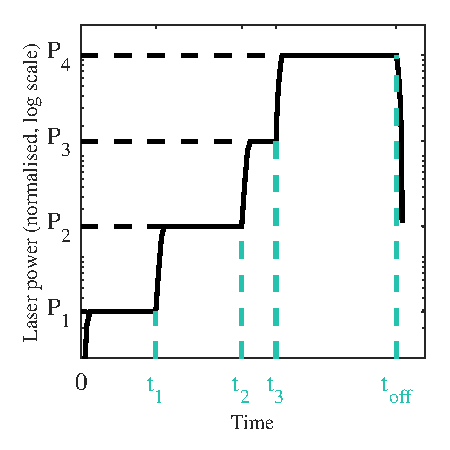
\includegraphics[width=.45\textwidth]{figures/LowCR/LaserProfile_half.eps}
\subfigure b)\includegraphics[width=.45\textwidth]{figures/LowCR/Capsule.pdf}
\caption{\label{fig:CapsuleAndLaserProfile}Plots of a) the laser profile and b) the capsule design. The laser sequence consists of four pulses of increasing power. The power begins to increase at the times $0, t_1, t_2$ and $t_3$ (with a linear rise over 200 \unit{\pico\second}), and the laser is switched off at time $t_{off}$ (with a linear decay over 200 \unit{\pico\second}). The capsule has three layers, with material interfaces at $R_{vapour}$ and $R_{foam}$ and an outer radius of $R_{capsule}$. When optimising this design, $R_{capsule}$ is selected and considered fixed. This is used to define the laser pulse powers $P_1, P_2, P_3$ and $P_4$, which are also not changed. This leaves seven optimisation parameters, which are indicated in teal: $t_1, t_2, t_3, t_{off}, R_{vapour}, R_{foam}$ and $\rho_{vapour}$ (the DT vapour density).}
\end{figure}

In order to perform the implosion optimisations, a general capsule design and laser pulse sequence were developed. These contained a number of free parameters which could then be varied in the optimisation. This section will describe the particular pulse profile and capsule design used.

The capsule, displayed in Figure \ref{fig:CapsuleAndLaserProfile}, was a simple three layer design consisting of a central DT-vapour region surrounded by a DT-wetted-foam layer and a deuterated plastic (CD) ablator. Optimisations were performed for a number of capsule outer radii - during the optimisation of each of these, the outer radius was treated as a fixed parameter The interior dimensions of the capsule ($R_{vapour}$ and $R_{foam}$) were varied during the optimisation, as was the density in the vapour region ($\rho_{vapour}$) (which was restricted to the 0.6 \unit{\milli\gram\per\centi\meter\cubed} $< \rho_{foam} <$ 4.0 \unit{\milli\gram\per\centi\meter\cubed} range achievable with wetted-foam capsules). The wetted-foam layer had a fixed density of 0.253 \unit{\gram\per\centi\meter\cubed}, while the ablator had a density of 1.04 \unit{\gram\per\centi\meter\cubed}. This represents a realistic capsule design similar to those used in previous experiments\footnote{ The use of a central vapour region surrounded by a dense fuel layer is standard for ignition designs, but the choice of ablator can vary: these can include the use of HDC rather than plastic \cite{Mackinnon2014}, or can contain layers of dopants (such as silicon) to absorb hot-electrons and thus minimise preheating \cite{Solodov2022}.}, with a minimal amount of complexity. 

The laser pulse profile, displayed in Figure \ref{fig:CapsuleAndLaserProfile}, consisted of a series of `steps' of constant laser power. A 351 \unit{\nano\meter} laser was used (corresponding to the third-harmonic of Nd:glass, as used at most ICF facilities), with a 0.2 \unit{\nano\second} linear rise time over which the changes in power occur. Both three- and four-pulse profiles were considered. The timings of each step ($t_1, t_2$ and $t_3$ in the figure) were treated as optimisation parameters, along with the time at which the laser was switched off ($t_{off}$). The relative laser powers were fixed and were not changed during the optimisation; ideally these would have also been varied, but it would have added significant complexity to the optimisation. The pulse-powers were chosen to roughly reduce the amount of entropy injected into the fuel. This laser profile was chosen for ease of optimisation, but again presents a simple realistic pulse profile that could be implemented on current facilities.

Optimisation campaigns were performed for a number of different capsule radii. For each radius, the intensity criteria determined the peak laser power, and the pulse profile was scaled accordingly. The different capsule radii produced implosions requiring different amounts of laser energy, since the radius determined both the laser power and the implosion time. The three laser timings, laser switch off time, two internal capsule radii and DT vapour density resulted in seven optimisation parameters.

\section{Performing the simulation campaign} \label{sec: OptimisationCampaign}

\subsection{The simulation code \texttt{HYADES}}

The 1D Lagrangian radiation hydrodynamics code \texttt{HYADES} was used to perform the simulations. \texttt{HYADES} is developed by Cascade inc., and was ran on the SCARF supercomputer at the UKRI-STFC Rutherford Appleton Laboratory. It has also previously been used for other large-scale simulation campaigns of ICF implosions \cite{Hatfield2019}. 

\texttt{HYADES} contains a number of different options for the various physics models. Those used in these simulations were based on the advice and recommendations of Dr Robbie Scott at the CLF, and are discussed in Section \ref{sec:additional-physics-in-fluid-codes}. A multiplier of 0.8 was also applied to the input laser energy to account for losses (such as those due to cross-beam energy transfer). A series of benchmarking simulations were performed after the main simulation campaign to confirm that these settings were sufficient to describe experimental shots; theses are described in the Appendix \ref{app:benchmark}.

The DT vapour regions were described in the simulations using the in-line \texttt{HYADES} QEOS model, while the thin deuterated-plastic shell used the SESAME EOS table for CH. These are the standard, accepted ways of describing these materials. The wetted-foam layer was less well-described, as no equation of state table for DT-wetted-foam was available. Instead, this layer was described as a pure-DT layer at the wetted-foam density, using the  DT QEOS model. This neglects the presence of the foam, and is a limitation of this work which is discussed further in later sections.

\subsection{Capsule meshing}

\texttt{HYADES} does not have an in-built meshing routine to discretise the capsule, and thus a meshing script had to be produced to allow different targets to be simulated. This mesh has two major requirements to ensure accuracy; the resolution of the mesh at the capsule outer edge should be sufficiently high, and the relative mass difference between zones should not be much greater than $\sim$ 2\%. In addition to this, an increased number of zones/mesh points leads to an increased simulation time, and thus it is desirable to keep the number of zones to a minimum while satisfying these two conditions.

A custom meshing routine was written for this simulation campaign. This routine was automatic and robust, allowing meshes to be created to describe capsules of a range of different sizes and layer thicknesses relevant to this investigation. The production of such a meshing algorithm was essential to being able to perform the large parameter scans that were the main feature of this work, as it enabled large numbers of capsules with different structures to be simulated with accuracy. The principles of this code (along with the underlying theory) is outlined in Appendix \ref{app:KeyCode}.

The meshing algorithm produced worked sufficiently well for the campaign to be conducted. It operated less well as the thicknesses of the layers began to vary too drastically, but this did not prevent the optimisations being performed; if the thicknesses had changed drastically enough that for the meshing code to stop working well, the performance had always decreased to such an extent that it was clearly not worth investigating, or the criteria for implosion velocity/IFAR would have been exceeded. However, if simulations of drastically different designs were required, a new and more robust meshing algorithm would need to be developed.

\subsection{Conducting the simulation campaign}

Separate optimisation campaigns were performed to optimise capsules of different outer radii. For each optimisation, a rough initial simulation was first performed. Large parameter scans were then performed varying either the two layer thicknesses, or two of the three laser timings, with roughly 100-200 simulations being performed in each scan. The results of these parameter scans would be identified, and implosions displaying the most promising criteria of the gain and the instability criteria selected. A new round of simulations would then be performed scanning over other parameters, and the process repeated. This was an iterative process - optimising the laser timings would then often lead to a new optimal thickness, which in turn would lead to a change in the optimal laser timings again. This process was repeated until no further improvement could be obtained.

Throughout the optimisation, the results would be monitored and the vapour density would also be investigated. For instance, if there were a number of capsules with lower yield than the current `optimal' design, but which also had a much lower convergence ratio than the limit of 16, then the vapour pressure would be reduced - this would increase the CR and gain of these capsules, and may result in them outperforming the previous best result. Equally, if a large number of the capsules satisfied the other criteria but the convergence ratio was too high, the vapour density would be reduced. This led to multiple repeats of the same round of optimisation at different vapour densities.

The time at which the laser was turned off was also treated separately from the other optimisation parameters. At some late time in each implosion continuing to apply the laser results in no benefit to the fusion performance, but it continues to cost energy and thus causes the gain to decrease. This effect can be substantial, and trends in the gain were being obscured based on how long after this point the laser was applied for. To resolve this, the laser was applied until the end of the each simulation, and the gain calculation was adjusted so that only the laser energy used up until the bang time was included in the calculation. This meant that the influence of this laser switch-off time was removed. Once the implosion had otherwise been optimised, the laser switch off-time would then be varied and the true gain (using the full applied laser energy) would be calculated; this would reveal a clear optimal value, and this would then be reported as the final gain for the optimised implosion.

Care was also taken to ensure that appropriate time resolution was being used in all simulations, and that the simulation end time was appropriate. If the simulation ended before the capsule had properly converged, the gain would inevitably be too low. This could typically be spotted by unfeasible data (for instance, a very low convergence ratio). To test for this, a representative number of the simulations would be analysed individually to check that the full behaviour was being captured, and that the simulations looked appropriate.

This procedure generated the `optimal' design for a particular capsule radius, and a particular number of laser pulses. The procedure was repeated multiple times to generate optimal 3-pulse and 4-pulse sequences for a range of different capsule radii.

\subsection{Hydroscaling}

When this campaign was first conducted (in 2020) it was done as described above for each capsule, in an attempt to minimise the number of assumptions on the optimal implosion. However, it was clear that all the optimised capsules had relatively comparable thicknesses and timings. In 2022, a further optimisation was performed to fill in a gap in the energies investigated, and this time hydrocaling relations were applied to produce an initial capsule from which to start the optimisation. This significantly reduced the rounds of simulations required to achieve convergence.

Hydroscaling makes use of the fact that much of the physics in an ICF implosion (particularly in 1D) is scale independent, and thus many of the parameters scale in a straightforward manner with capsule size. These relations state that $t \propto R \propto E^{1/3}$ where $t$ and $R$, are the implosion timings (including all laser timings) and capsule radii (including all internal boundaries) respectively, and $E$ is the laser energy \cite{Nora2014}. This meant that, based on the energy desired for the implosion, a rough estimate could be produced of the necessary capsule size. The interior dimensions of the capsule could be scaled accordingly, as could the laser timings. This was then used as the starting point of the optimisation to produce a capsule that already had a good level of fusion performance, which was then further increased by the optimisation.

\section{Results and analysis} \label{sec: LowCRResults}

Over 20,000 simulations were performed in total, with over 10,000 satisfying all four instability criteria; these $\sim$10,000 valid simulations are plotted as a function of gain vs laser energy in Figure \ref{fig:loglog}. The data can be seen to form eight rough peaks, corresponding to the eight different outer radii (and thus energy scales) considered. The four-pulse laser sequences are displayed in black, while the three-pulse sequences are displayed in teal. As expected, the lower adiabat four-pulse sequences outperformed the three-pulse sequences at all energy scales. The best performing three-pulse and four-pulse simulations for each capsule size have been tabulated in Table \ref{tab:ThirdHarmonic}. 

\begin{figure}[ht!]
\centering
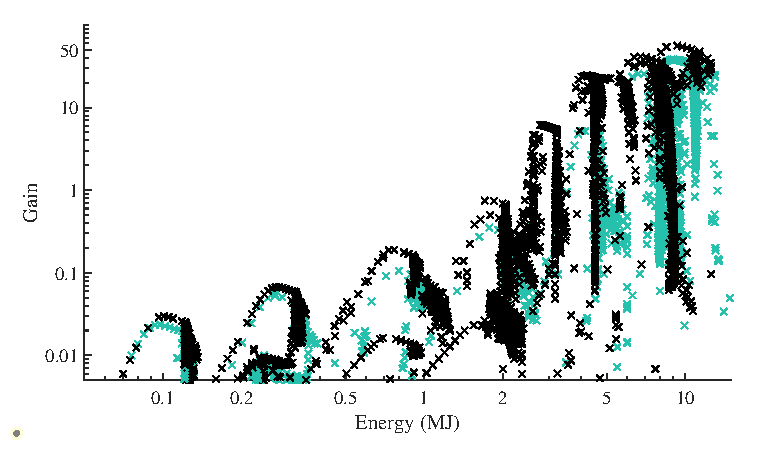
\includegraphics{figures/LowCR/AllData_full.eps}
\caption{A log-log plot showing the simulated gain vs input energy for all simulations satisfying the low-instability criteria. Those using a three-pulse sequence are displayed in teal, while those using a four-pulse sequence are displayed in black. The simulations form eight rough peaks, corresponding to the eight different capsule sizes.}
\label{fig:loglog}
\end{figure}


\begin{table}
\resizebox{\textwidth}{!}{%
  \centering
\begin{tabular}{|c|c|c|c|c|c|c|c|c|}
\hline
 Number of pulses & \multicolumn{8}{c|}{3} \\
 \hline
 Size multiplier & 0.25 & 0.35 & 0.5 & 0.65 & 0.75 & 0.85 & 1 & 1.1 \\ 
\hline
Laser energy (MJ) & - & - & 0.80 & 1.8 & - & 4.0 & 6.6 & 8.9\\ 
Gain & - & - & 0.11 & 0.35 & - & 5.2 & 26 & 38\\ 
Convergence ratio & - & - & 15.3 & 15.5 & - & 15.9 & 16.0 & 16.0\\ 
IFAR & - & - & 20.3 & 18.7 & - & 15.2 & 14.3 & 12.7 \\ 
Implosion velocity (km/s) & - & - & 399.2 & 395.4 & - & 373.9 & 358.4 & 332.4\\ 
Max pulse power (TW) & - & - & 173.00 & 292.38 & - & 500.12 & 692.13 & 837.50\\ 
Pulse 2 switch on time (ns) & - & - & 3.65 & 3.80 & - & 5.00 & 6.20 & 7.00\\ 
Pulse 3 switch on time (ns) & - & - & 4.15 & 4.90 & - & 6.30 & 7.60 & 8.80\\ 
Laser switch off time (ns) & - & - & 8.50 & 10.50 & - & 13.75 & 16.50 & 18.60\\ 
Vapour/liquid boundary (\si[per-mode=symbol]{\milli\meter}) & - & - & 1.3000 & 1.6835 & - & 2.2100 & 2.6100 & 2.8710\\ 
Liquid/CD boundary (\si[per-mode=symbol]{\milli\meter}) & - & - & 1.4000 & 1.8200 & - & 2.3800 & 2.7900 & 3.0580\\ 
Outer radius (\si[per-mode=symbol]{\milli\meter}) & - & - & 1.4250 & 1.8525 & - & 2.4225 & 2.8500 & 3.1350\\ 
Vapour density (\si[per-mode=symbol]{\milli\gram\per\centi\meter\cubed}) & - & - & 1.00 & 0.85 & - & 0.65& 0.65 & 0.70\\
\hline

Number of pulses & \multicolumn{8}{c|}{4} \\
\hline
Size multiplier & 0.25 & 0.35 & 0.5 & 0.65 & 0.75 & 0.85 & 1 & 1.1 \\ 
\hline
Laser energy (MJ) & 0.10  & 0.27 & 0.77 & 1.7 & 2.8 & 4.2 & 6.7 & 8.5\\ 
Gain & 0.030 & 0.067 & 0.19 & 0.75 & 6.1 & 24 & 42 & 54\\ 
Convergence ratio & 15.7 & 15.7 & 16.0 & 15.8 & 16.0 & 15.9 & 16.0 & 15.7\\ 
IFAR & 23.4 & 27.5 & 29.7 & 25.1 & 23.8 & 21.2 & 18.4 & 15.7\\ 
Implosion velocity (km/s) & 391.4 & 395.8 & 399.6 & 399.6 & 387.8 & 347.5 & 334.1 & 311.0\\ 
Max pulse power (TW) & 43.26 & 84.79 & 173.00 & 292.38 & 389.36 &500.12 & 692.13 & 837.50\\ 
Pulse 2 switch on time (ns) & 1.10 & 2.20 & 2.60 & 3.60 & 4.20 & 3.70 & 5.20 & 5.70\\ 
Pulse 3 switch on time (ns) & 3.00 & 4.60 & 5.60 & 7.80 & 8.80 & 9.40 & 12.80 & 15.00\\ 
Pulse 4 switch on time (ns) & 3.60 & 5.50 & 6.80 & 9.50 & 10.90 & 11.40 & 15.30 & 18.00\\ 
Laser switch off time (ns) & 5.80 & 8.50 & 11.00 & 15.00 & 17.65 & 19.40 & 24.50 & 27.50\\ 
Vapour/liquid boundary (\si[per-mode=symbol]{\milli\meter}) & 0.6325 & 0.8950 & 1.3050 & 1.6705 & 1.9275 & 2.2100 & 2.6000 & 2.8270\\ 
Liquid/CD boundary (\si[per-mode=symbol]{\milli\meter}) & 0.69625 & 0.976 & 1.3950 & 1.8200 & 2.1000 & 2.3630 & 2.7800 & 3.0580\\ 
Outer radius (\si[per-mode=symbol]{\milli\meter}) & 0.7125 & 0.9975 & 1.4250 & 1.8525 & 2.1375 & 2.4225 & 2.8500 & 3.1350\\ 
Vapour density (\si[per-mode=symbol]{\milli\gram\per\centi\meter\cubed}) & 1.35 & 1.35 & 1.05 & 1.00 & 0.90 & 0.85 & 1.00 & 1.00\\
\hline
\end{tabular}}
\caption{Simulation parameters for the best performing three and four-pulse laser sequences for a range of capsule radii. The first optimised capsule was that with a size multiplier of 1. In order to keep $I\lambda^2$ constant as a function of capsule radius, the pulse powers are multiplied by the square of the size multiplier. A higher level of precision is provided for many quantities than would be expected for 1D simulations, in order to show how the parameters compare to the low-instability criteria. While convergence ratio is in places displayed as 16.0, the value to the precision calculated in the analysis is below this upper limit. The original simulation campaign was performed for five capsule sizes; three further sizes (0.25, 0.35 and 0.75) were performed later, but only four pulse sequences were optimized.}
\label{tab:ThirdHarmonic}
\end{table}

These results demonstrate that high reactor-level gains can be achieved in this regime, with a gain of 54 being achieved for an energy of 8.5 \unit{\mega\joule}. However, this is a much higher energy than is currently achievable, and is likely too high for an economically viable fusion reactor - suggesting that a fusion reactor could not be constructed using this particular approach. However, the lower energy performance is interesting. The gains of 0.19 and 0.75 at 0.77 \unit{\mega\joule} and 1.7 \unit{\mega\joule} respectively are impressive given the conservative nature of this regime. It is also worth noting that when this work was performed the record ICF gain was 0.03, and so this result suggested an improvement (at the time) of an order of magnitude over the then-current standard. Recent experiments have achieved high gains, but this work suggests that comparable performance can be achieved in this regime where instability growth is less of a concern (and implosions would hopefully be robust). The recent NIF results (a gain of 0.7 at 1.9 MJ, and a gain of 1.5 at 2.05 MJ) actually fit just below the trend of this data (this is plotted in Figure \ref{fig:ArF and Two colour} in the following chapter), suggesting that the performance predicted here is comparable to the current record shots on the NIF.

The conditions in the hotspot and shell of the 0.77 \unit{\mega\joule} capsule are displayed in \ref{fig:HSandShellLMJ}. It can be seen that the hotspot conditions are close to that required for ignition. The areal density is greater than the 0.3 \unit{\gram\per\centi\meter\squared} commonly quoted as required for ignition to occur, but the ion temperature (just below 4 keV) is slightly too low. This suggests that ignition could be within reach, if it was possible to increase this ion temperature just prior to the bang-time. This is investigated further in Chapter \ref{ch-FurtherSims}. It is also interesting to note the relatively low areal density of the shell, which arises from the limited convergence of the capsule. This is most easily increased in this regime by increasing the size of the capsule.

It is useful to note again here the purpose of this work, which is not to claim that these exact gains are possible - these are the results of 1D simulations only, and thus can not be expected to be fully accurate. However, the expected low-instability growth means that such simulations are expected to be a more representative estimate of performance than would otherwise be the case, and thus should be sufficient to give a good first-estimate of potential experimental performance. Overall, these results show that it may indeed be possible to achieve interesting fusion performance (comparable to the current best-performing shots on the NIF) in this regime, based around low-convergence ratio and where performance is expected to be minimal.

\begin{figure}[ht]
\centering
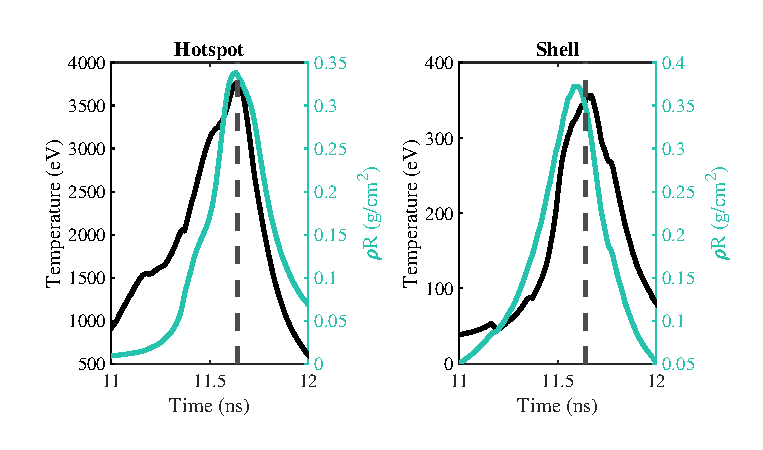
\includegraphics{figures/LowCR/RhoRandT.eps}
\caption{Plots displaying the temperature (black) and areal density (teal) in the hotspot and shell for the 0.77 \unit{\mega\joule} implosion.}
\label{fig:HSandShellLMJ}
\end{figure}


\section{Limitations and suggested future work} \label{sec: LowCRLimitations}
There are a number of limitations of this work, some of which will be investigated further in the following chapters. These limitations also suggest some potential avenues for future research.

The fundamental limitation of this work is the use of 1D simulations. While the effort made here to define a low-instability regime means that 1D like-behaviour is expected, this is still a fundamental and untested assumption upon which this work relies. While 1D simulations are sufficient for an initial investigation of the regime, simulations in higher dimensions are required to estimate the level of instabilities that may be present. We have recently secured access to the University of Rochester's RIGEL code, and are collaborating with them to perform confirmatory 2D simulations.

The direct-drive nature of this work coupled with the high laser energies makes experimental verification of the regime challenging. When this work was performed, the use of cryogenic targets and the high energies meant that performing shots based on these designs would not be possible, due to a lack of cryogenic capabilities for direct-drive shots at the NIF \cite{Hohenberger2015}. Fortunately this has since been rectified, and direct-drive shots of wetted-foam targets are being planned. However, this still requires cryogenic shots on the NIF, which makes limits the opportunity to test this regime. An alternative solution to this is proposed in the next chapter. In addition, such shots would need to be performed in a PDD configuration. This is contrary to these simulations, where fully symmetric direct-drive was assumed (and the benchmarking simulations in Appendix \ref{app:benchmark} suggest that a reduced laser input multiplier would potentially be required to describe PDD shots).

Thirdly, the simulations make a number of approximations that are not particularly accurate, which likely lead to some over-estimation of the performance. The two main ones are as follows: 1) the laser in the 1D simulations is focussed at the centre of the capsule, which means that it remains perfectly focused as the capsule implodes. This is unphysical. However, the benchmarking simulations in Appendix \ref{app:benchmark} suggest that the input multiplier used to account for laser losses (such as due to this effect) is reasonable for the case of a spherical direct-drive implosion, although a lower multiplier may be required for a polar direct drive setup. 2) The description of the wetted foam as simply a DT layer (with the CH foam not accounted for) is a poor one, and is only valid if the foam density is below $\sim10$~\si[per-mode=symbol]{\milli\gram\per\centi\meter\cubed} \cite{CHFoamLim}. Other groups have used a less-compressible mixed CH + DT equation of state to describe this material with more accuracy \cite{Olson2021}; this is investigated in the following section. This is further complicated by the fact that the equation of state for even dry foams at these low densities are not well simulated, which motivated the experiment in later chapters. Further study is required to better describe this material if wetted-foams are to be simulated to higher accuracy, and ultimately experiments to measure the wetted foam equation of state are required; this is another topic that we are continuing to investigate.

In addition, while these are presented as `optimisation' campaigns, exploring such large parameter spaces manually is incredibly difficult, and thus no guarantee can be made that optimal performance has been obtained. This approach would be well-suited to a machine learning approach, which could automate the optimisation process and hopefully explore the parameter space more efficiently. Machine-learning has been applied to ICF for similar problems in the past successfully \cite{Hatfield2019}, and this is something that we are currently investigating within our research group. If this could be done successfully, it would allow many more simulation campaigns to be performed of this ilk with relative ease. The impact of more parameters could be explored (for example, the laser pulse powers), and the criteria applied to limit the parameter space could be adjusted (i.e. to investigate alternative maximum implosion velocities) or to include other parameters (for instance, applying a minimum permitted adiabat).

In addition, while the regime identified is expected to be result in low-instability growth, there are other parameters which could be included to increase confidence in this. The most obvious would be the adiabat of the implosion. In addition, no limit was placed on the strength of the first shock, as the impact of particular asymmetry seeds was not considered in this work. This is a significant limitation, since the strength of the first shock has been shown to be key to mitigating instabilities from the support tent (in indirect-drive implosions) and ablator micro-structure. If future simulation campaigns were to be performed (particularly if machine learning was to be applied), repeating this campaign with a 10 Mbar first shock should be a priority.

\section{Conclusion} \label{sec:LowCRConclusions}
A simulation campaign to investigate the performance of wetted-foam capsules in a low-instability regime was presented, where the regime is defined by limits to convergence ratio, IFAR, implosion velocity, and laser intensity. While the laser energy necessary for an IFE reactor based on this approach is not feasible, the performance at lower energies is comparable to the recent record shots on the NIF. This suggests that substantial fusion performance can be obtained despite the conservative approach taken here, and that further exploration of this regime could be interesting. A variety of potential extensions and improvements to this work have been suggested, many of which are explored in the following chapter.

This chapter has also demonstrated the utility of this style of optimisation campaign - a general platform which can be used to explore fusion performance in a particular parameter space. This approach has again been applied in the subsequent chapter to explore variations on the implosion scheme discussed here.





















%\begin{table}[t]
%\resizebox{\textwidth}{!}{%
%\centering
%\begin{tabular}{|c|c|c|c|c|c|c|}
%\hline
% Number of pulses & \multicolumn{6}{c|}{3} \\
% \hline
% Size multiplier & 0.5 & 0.65 & 0.75 & 0.85 & 1 & 1.1 \\ 
%\hline
%Laser energy (MJ) & 0.80 & 1.8 & - & 4.0 & 6.6 & 8.9\\ 
%Gain & 0.11 & 0.35 & - & 5.2 & 26 & 38\\ 
%Convergence ratio & 15.3 & 15.5 & - & 15.9 & 16.0 & 16.0\\ 
%IFAR & 20.3 & 18.7 & - & 15.2 & 14.3 & 12.7 \\ 
%Implosion velocity (km/s) & 399.2 & 395.4 & - & 373.9 & 358.4 & 332.4\\ 
%Max pulse power (TW) & 173.00 & 292.38 & - & 500.12 & 692.13 & 837.50\\ 
%Pulse 2 switch on time (ns) & 3.65 & 3.80 & - & 5.00 & 6.20 & 7.00\\ 
%Pulse 3 switch on time (ns) & 4.15 & 4.90 & - & 6.30 & 7.60 & 8.80\\ 
%Laser switch off time (ns) & 8.50 & 10.50 & - & 13.75 & 16.50 & 18.60\\ 
%Vapour/liquid boundary (\si[per-mode=symbol]{\milli\meter}) & 1.3000 & 1.6835 & - & 2.2100 & 2.6100 & 2.8710\\ 
%Liquid/CD boundary (\si[per-mode=symbol]{\milli\meter}) & 1.4000 & 1.8200 & - & 2.3800 & 2.7900 & 3.0580\\ 
%Outer radius (\si[per-mode=symbol]{\milli\meter}) & 1.4250 & 1.8525 & - & 2.4225 & 2.8500 & 3.1350\\ 
%Vapour density (\si[per-mode=symbol]{\milli\gram\per\centi\meter\cubed}) & 1.00 & 0.85 & - & 0.65& 0.65 & 0.70\\
%\hline

%Number of pulses & \multicolumn{6}{c|}{4} \\
%\hline
%Size multiplier & 0.5 & 0.65 & 0.75 & 0.85 & 1 & 1.1 \\ 
%\hline
%Laser energy (MJ) & 0.77 & 1.7 & 2.8 & 4.2 & 6.7 & 8.5\\ 
%Gain & 0.19 & 0.75 & 6.1 & 24 & 42 & 54\\ 
%Convergence ratio & 16.0 & 15.8 & 16.0 & 15.9 & 16.0 & 15.7\\ 
%IFAR & 29.7 & 25.1 & 23.8 & 21.2 & 18.4 & 15.7\\ 
%Implosion velocity (km/s) & 399.6 & 399.6 & 387.8 & 347.5 & 334.1 & 311.0\\ 
%Max pulse power (TW) & 173.00 & 292.38 & 389.36 &500.12 & 692.13 & 837.50\\ 
%Pulse 2 switch on time (ns) & 2.60 & 3.60 & 4.20 & 3.70 & 5.20 & 5.70\\ 
%Pulse 3 switch on time (ns) & 5.60 & 7.80 & 8.80 & 9.40 & 12.80 & 15.00\\ 
%Pulse 4 switch on time (ns) & 6.80 & 9.50 & 10.90 & 11.40 & 15.30 & 18.00\\ 
%Laser switch off time (ns) & 11.00 & 15.00 & 17.65 & 19.40 & 24.50 & 27.50\\ 
%Vapour/liquid boundary (\si[per-mode=symbol]{\milli\meter}) & 1.3050 & 1.6705 & 1.9275 & 2.2100 & 2.6000 & 2.8270\\ 
%Liquid/CD boundary (\si[per-mode=symbol]{\milli\meter}) & 1.3950 & 1.8200 & 2.1000 & 2.3630 & 2.7800 & 3.0580\\ 
%Outer radius (\si[per-mode=symbol]{\milli\meter}) & 1.4250 & 1.8525 & 2.1375 & 2.4225 & 2.8500 & 3.1350\\ 
%Vapour density (\si[per-mode=symbol]{\milli\gram\per\centi\meter\cubed}) & 1.05 & 1.00 & 0.90 & 0.85 & 1.00 & 1.00\\
%\hline
%\end{tabular}}
%\caption{Simulation parameters used to achieve the maximum gains for each capsule size for both pulse sequences. The original capsule was the column with size multiplier of 1. New capsule sizes (and thus energy scales) were simulated by multiplying the radius by the size multiplier. In order to keep $I\lambda^2$ constant over different capsule sizes, the pulse powers were then multiplied by the square of the size multiplier. Gain is given to two significant figures, whilst convergence ratio, IFAR and implosion velocity are given to one decimal place. This level of precision is higher than would typically be quoted for a 1D simulation, but is used here to indicate how the values compare with the imposed limits. While convergence ratio is in places displayed as 16.0, the value to the precision calculated in the analysis is below this upper limit.}
%\label{tab:ThirdHarmonic}
%\end{table}

%\begin{table}[t]
%\centering
%\begin{tabular}{|c|c|c|c|}
%\hline
%Number of pulses & \multicolumn{3}{c|}{4} \\
%\hline
%Size multiplier & 0.25 & 0.35 & 0.75 \\ 
%\hline
%Laser energy (MJ) & 0.10  & 0.27  & 2.8\\ 
%Gain & 0.030 & 0.067 &  6.1\\ 
%Convergence ratio & 15.7 & 15.7 &  16.0\\ 
%IFAR & 23.4 & 27.5 & 23.8\\ 
%Implosion velocity (km/s) & 391.4 & 395.8 & 387.8\\ 
%Max pulse power (TW) & 43.26 & 84.79 & 389.36\\ 
%Pulse 2 switch on time (ns) & 1.10 & 2.20 & 4.20\\ 
%Pulse 3 switch on time (ns) & 3.00 & 4.60 & 8.80\\ 
%Pulse 4 switch on time (ns) & 3.60 & 5.50 & 10.90\\ 
%Laser switch off time (ns) & 5.80 & 8.50 & 17.65\\ 
%Vapour/liquid boundary (\si[per-mode=symbol]{\milli\meter}) & 0.6325 & 0.8950 & 1.9275\\ 
%Liquid/CD boundary (\si[per-mode=symbol]{\milli\meter}) & 0.69625 & 0.976 & 2.1000\\ 
%Outer radius (\si[per-mode=symbol]{\milli\meter}) & 0.7125 & 0.9975 & 2.1375\\ 
%Vapour density (\si[per-mode=symbol]{\milli\gram\per\centi\meter\cubed}) & 1.35 & 1.35 & 0.90\\
%\hline
%  \end{tabular}
%\caption{Simulation parameters used to achieve the maximum gains for three further capsules. These optimisations were done after the main campaign. The three-pulse sequences for these capsules were not fully optimised, and so have not been tabulated.}
%\label{tab:ThirdHarmonic_2}
%\end{table}